\documentclass[12pt,a4paper]{report}
\usepackage[utf8]{inputenc}
\usepackage{amsmath}
\usepackage{amsfonts}
\usepackage{amssymb}
\usepackage{graphicx}
\usepackage{hyperref}
\usepackage{float}

\renewcommand\thesection{\arabic{section}.}

\begin{document}
	
	\section{Brief Description}
	
	This project is an implementation of a simple space game with a straightforward user interaction. It consists of a spaceship, a star and an asteroid system. The physics is basic and only used for animation purposes. Currently, no interaction, such as collisions, between different models in the game is implemented.
	
	\section{Building blocks}
	
	For the implementation of the visualization of the elements of the game, \textit{three.js} library is used. The model of the spaceship is a low polygonal model designed in Blender. The star is implemented as a sphere with randomized bump map with texture obtained from wikipedia (sun texture image). Each asteroid is randomly generated with different sizes and bumps for each. 
	
	\section{Model hierarchy}
	
	The scenery consists of main star, an asteroid belt with user defined number of asteroids (you can change it in the code), and the spaceship. The ship consists of fuselage, left and right wings, and left and right engines. These engines are warp-drive like, so enabling them turn on the point light representing the engine blast. 
	
	The hierarchy of the complete scenery is given in the following figure:
	
	\begin{figure}[H]
		\centering
		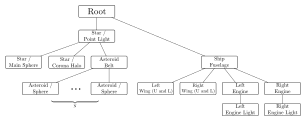
\includegraphics[width=1.1\linewidth]{img/hierarchy}
		\caption{Model hierarchy}
		\label{fig:hierarchy}
	\end{figure}
	
	This kind of hierarchy enables the simulation of real -- world scenario: the star rotates independently, asteroids rotate around the star, and the ship cruises within this star system. This is obviously not a true Newtonian dynamics of the star, star system and the ship moving around the star, but represents a good approximation of it. For example, ship should rotate around the star's orbit, but this is not implemented.
	
	\section{Textures and Lights}
	
	\subsection{Textures}
	
	The textures are used for the star and asteroids. Both of these textures are taken from Wikipedia, so they are under Creative Commons license. For the start, I used the texture of our Sun shown in the following figure:
	
	 \begin{figure}[H]
	 	\centering
	 	\includegraphics[width=0.9\linewidth]{img/sun}
	 	\caption{Sun texture model}
	 	\label{fig:sun}
	 \end{figure}
 
 	Furthermore, a slight bump map was added to the star model using this texture image. I simply converted the image to grayscale and intensified some colors, while decreasing the value of others. You can check the image in the source tree of the project (textures folder).
 	
 	Asteroids are implemented as randomized spheres. This is done by setting arguments for SphereGeometry class in three.js, horizontal segments (), vertical segments and radius. Similarly, the following texture from Wikipedia is used for asteroids:
 	
 	\begin{figure}[H]
 		\centering
 		\includegraphics[width=0.9\linewidth]{img/asteroid}
 		\caption{Asteroid texture model}
 		\label{fig:asteroid}
 	\end{figure}
 
 	Likewise, the bump map was created from this texture image by applying similar steps as with a sun's texture.	
 	
 	\subsection{Lights}
 	
 	The following lights are added to the model:
 	
 	\begin{itemize}
 		\item Ambient light for added light to the scene (unrealistic physically, but makes everything more visible)
 		\item Point light for the left engine
 		\item Point light for the right engine
 		\item Point light for the start
 		\item Point light as a dummy light for the asteroid belt (intensity set to 0)
 	\end{itemize}
	
	\section{User Interactions}
	
	User interactions are divided into two parts:
	
	\begin{itemize}
		\item Ship interactions
		\item Camera interactions
	\end{itemize}

	For the ship interactions, you can rotate the wings (although this does not changes the physics, just implemented as an eye candy), engage the engines (which increases the thrust significantly) and turns of the engine lights, and you can use the arrow keys: up/down for increasing/decreasing the thrust slightly, left/right for rotating.
	
	Camera interactions are available as well, enabling the use of three camera types: first as a third-person-view, second as a above-cockpit view, and the third for orbital movement around the scene using the computer mouse.
	
	\section{Animations}
	
	The following animations are implemented:
	
	\begin{itemize}
		\item Star rotation
		\item Asteroid belt rotation around the star
		\item Wing rotations when engaging the wings of the spaceship
	\end{itemize}

	All animations are implemented naively using pure JavaScript. This is done by counting the iterations of the hole scenery (renderer ticks) and designing the animations accordingly by setting the start and stop ticks.	
	
	\section{User Manual}
	
	The project requires web browser and a simple web server. This is due to the restrictions modern web browser impose on loading local files, i.e. 3D meshes and textures from local storage.
	
	The simplest one is \textit{http.server} from the standard Python 3 library. Run the following command:
	
	\begin{verbatim}
		$ python3 -m http.server
	\end{verbatim}
	
	from the root folder of the project (where \textit{index.html} is located). The following resulting code will appear:
	
	{\footnotesize
	\begin{verbatim}
		Serving HTTP on 0.0.0.0 port 8000 (http://0.0.0.0:8000/) ...
		127.0.0.1 - - [24/Jul/2021 21:40:30] "GET / HTTP/1.1" 200 -
		127.0.0.1 - - [24/Jul/2021 21:40:30] "GET /js/main.js HTTP/1.1" 200 -
		127.0.0.1 - - [24/Jul/2021 21:40:33] "GET /obj/ship2.gltf HTTP/1.1" 200 -
		127.0.0.1 - - [24/Jul/2021 21:40:33] "GET /obj/wing.gltf HTTP/1.1" 200 -
		127.0.0.1 - - [24/Jul/2021 21:40:33] "GET /obj/engine.gltf HTTP/1.1" 200 -
		127.0.0.1 - - [24/Jul/2021 21:40:33] "GET /textures/sun.jpg HTTP/1.1" 200 -
		127.0.0.1 - - [24/Jul/2021 21:40:33] "GET /textures/sun_bump.jpg HTTP/1.1" 200 -
		127.0.0.1 - - [24/Jul/2021 21:40:33] "GET /textures/asteroid.jpg HTTP/1.1" 200 -
		127.0.0.1 - - [24/Jul/2021 21:40:33] "GET /textures/asteroid_bump.jpg HTTP/1.1" 200 -
		127.0.0.1 - - [24/Jul/2021 21:40:36] code 404, message File not found
		127.0.0.1 - - [24/Jul/2021 21:40:36] "GET /favicon.ico HTTP/1.1" 404 -
	\end{verbatim} }
	
	This means that the web server is \textit{serving} the files required for \textit{index.html} to properly run the game. Open the \url{http://localhost:8000} in the web browser and the following will appear:
	
	\begin{figure}[H]
		\centering
		\includegraphics[width=0.9\linewidth]{img/screen}
		\caption{Start screen of the game}
		\label{fig:screen}
	\end{figure}

	To interract with the game, the following keys are available:
	
	\begin{itemize}
		\item KeyUP - go faster
		\item KeyDOWN - slow down
		\item KeyLEFT - turn left
		\item KeyRIGHT - turn right
		\item D - fire up/turn off engines to go really fast
		\item W - wings on/off with a simple animation
		\item 1 - third person view camera
		\item 2 - cockpit view camera
		\item 3 - camera with orbital control (mouse)
	\end{itemize}
	
	
\end{document}